\chapter{Escales Logar\'{\i}tmiques} \index{escales logar\'{\i}tmiques}

En diferents camps de l'electrot\`{e}cnia, \'{e}s usual trobar-se gr\`{a}fics amb escales
logar\'{\i}tmiques.

Un exemple clar, s\'{o}n els gr\`{a}fics d'actuaci\'{o} dels interruptors magnetot\`{e}rmics o dels
fusibles, on les seves corbes caracter\'{\i}stiques intensitat--temps estan representades en
una escala logar\'{\i}tmica--logar\'{\i}tmica o lineal--logar\'{\i}tmica.

En aquests casos, es presenta freq\"{u}entment la necessitat de determinar amb exactitud un
punt de la corba, que no coincideix amb cap de les l\'{\i}nies divis\`{o}ries del gr\`{a}fic. Atenent a
la Figura \vref{pic:escala log}, es tractaria de determinar el valor $x$ dins de la d\`{e}cada
$10^N$ a $10^{N+1}$.

\begin{figure}[htb]
\vspace{5mm} \centering
    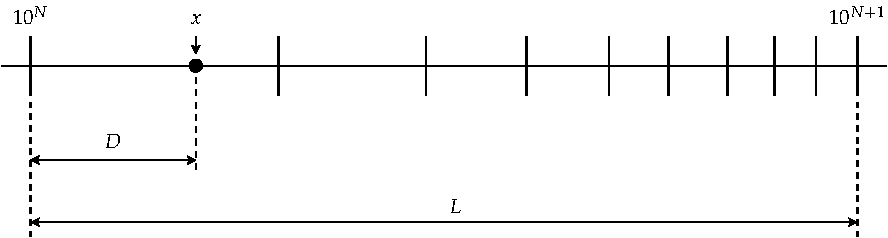
\includegraphics{Imatges/Ape-EscalesLog.pdf}
\caption{Escala logar\'{\i}tmica} \label{pic:escala log}
\end{figure}

Si mesurem amb un regle la dist\`{a}ncia $D$ des de l'inici de la d\`{e}cada fins al punt $x$, i
la longitud total $L$ de la d\`{e}cada, el valor $x$ buscat ve donat per l'expressi\'{o}:
\begin{equation}
    x = 10^{\left(N+\frac{D}{L}\right)}
\end{equation}

Si estem interessats en el problema invers, \'{e}s a dir, en  trobar la dist\`{a}ncia $D$
corresponent a un valor conegut $x$ dins de la d\`{e}cada $10^N$ a $10^{N+1}$, podem emprar
l'expressi\'{o}:
\begin{equation}
    D = L(\log x - N) = L \log\frac{x}{10^N}
\end{equation}

\begin{exemple}
Es tracta de trobar el valor $x$ dins de la d\`{e}cada 100 a 1000, corresponent a una
dist\`{a}ncia $D=11\unit{mm}$; la longitud total de la d\`{e}cada \'{e}s $L=56\unit{mm}$.

En aquest cas tenim $N=2$, i per tant:
\[
    x = 10^{\left(2+\frac{11\unit{mm}}{56\unit{mm}}\right)}= 157{,}19
\]
\end{exemple}

\begin{exemple}
Es tracta de trobar la dist\`{a}ncia $D$ a la qual hem de dibuixar el valor $x=5$, dins de la
d\`{e}cada 1 a 10; la longitud total de la d\`{e}cada \'{e}s $L=56\unit{mm}$.

En aquest cas tenim $N=0$, i per tant:
\[
    D = 56\unit{mm} \cdot (\log 5 - 0)  = 39{,}1\unit{mm}
\]
\end{exemple}
